%!TEX program = xelatex

\documentclass[11pt]{article}

\usepackage{hyperref}
\usepackage{graphicx}
\usepackage{wrapfig}
\usepackage{amssymb}
\usepackage{amsmath}
\usepackage{titlesec}
\usepackage{wrapfig}
\usepackage{caption}
\usepackage{subcaption}
\usepackage{sidecap}
\usepackage{clrscode}
\usepackage{xcolor}
\usepackage{float}
\usepackage{stackengine}

\usepackage[margin=0.75in]{geometry}

\newlength{\tindent}
\setlength{\tindent}{\parindent}
\setlength{\parindent}{0pt}
\renewcommand{\indent}{\hspace*{\tindent}}
\floatplacement{figure}{H}

\newcommand\tab[1][1cm]{\hspace*{#1}}
\newcommand{\SK}{\textbf{[SK]}\tab}
\newcommand{\KY}{\textbf{[KY]}\tab}
\newcommand{\CO}{\textbf{[CO]}\tab}
\newcommand\cdate[1][1cm]{\textbf{[#1]}}

\renewcommand{\thesubsection}{\thesection.\alph{subsection}}
\titleformat{\subsection}[runin]{\normalfont\large\bfseries}{\thesubsection}{1em}{}

\begin{document}

\begin{centering}
\Large
    \textbf{Bayesian Clustering and Topic Modeling of Gene Expression Data}  \\
    \vspace{2mm}
    \normalsize
    Skanda Koppula (\url{skoppula@mit.edu}), Karren Yang (\url{karren@mit.edu}) \\
    \vspace{2mm}
    \normalsize
    6.882 Project Proposal, \today \\
\end{centering}
\vspace{5mm}

\section{Overview}

We have made preliminary assessments of three topic models -- LDA, the Hierarchical Dirichlet Process (HDP), and the Indian Buffet Process Compound Dirichlet Process (IDP-DP) -- for discovering topics in single-cell RNA-sequencing (scRNA-seq) data. In this context, topics are sets of genes that are co-expressed across cells (i.e. gene modules) \footnote{The genes in gene modules generally move in tandem: so when a gene module is upregulated, all genes have higher expression. This motivates our use of topic models to capture these relationships.}. Since we would like topics to correpond to biologically useful gene modules, our main evaluation metric is the correpondence of the learned topics to known functional gene sets curated from literature (i.e. from the \texttt{MSigDB} database). While HDP and the IBP-DP offer greater flexibility in that the number of topics does not have to be defined a priori, we do not find evidence that they yield significantly more coherent topics; moreover, we find in practice that training the models and tuning the hyper-parameters to maintain a reasonable number of topics is less time-efficient than applying LDA over a range of number of topics. Moving forward, we will focus on implementing and evaluating a unified framework for clustering and topic modeling based on LDA. 

\section{Results}
\subsection*{Running LDA}

We explored two implementations of posterior inference for LDA on large datasets: one using online mean-field variational bayes for posterior estimate \cite{ovb, online}, and a broken \texttt{C++} Gibbs sampler for LDA that we modified to work \cite{plda}. We were able to get this latter sampler running parallel across multiple cores, with a burn-in of 100 iterations. We compare these two posterior estimation approaches using our entire dataset, with a 10\% held-out testing partition. We experimented with
$k=5, 10, 25, 50$ topics. \\

\iffalse
It was nececssary to use these implementations as we were unable to obtain any results using Python's out-of-the-box implementation of \texttt{lda} \cite{lda}. With our 250 MB dataset, the collapsed Gibbs sampler used in the implementation was taking too long to produce samples, even on larger server-grade machines and with a small number of LDA clusters. We explored modifying the source to parallelize the sampling, but found the source to be crabbed and hard to follow. \\
\fi

Figure \ref{fig:time} shows the time to complete each estimation method. As expected, Gibbs scales poorly with the parameter dimensionality and is strictly worse than online variational Bayes across all studied topic counts. We also calculated perplexity and log-likelihood for the OVB parameters, and very surprisingly, we found that log-likelihood decreased as number of topics increased on a held-out test set (Figure \ref{fig:ll}). We are currently trying to understand whether this is because of programming error.

\subsection*{Evaluating Biological Significance of LDA Topics}

We did gene set enrichment analysis using the minimum hypergeometric test \cite{hg} to compare our topics, which are ranked lists of genes, with existing collections of genes catalogued in the comprehensive gene module database, \texttt{MSigDB} \cite{msigdb}. Figure \ref{fig:pathways} in the Appendix shows topic-to-\texttt{MSigDB} module matches for which the $p$-value of the match is at least less than 0.3. Models with more topics tended to have more matches with higher significance. These results suggest that we need to train the model with more topics. We note that the $p$-values do \textit{not} factor for multiple hypothesis corrections, so at the moment we are only using them as relative measures of model quality.


\subsection*{LDA vs. HDP}

We trained an HDP topic model and compared it to LDA models with similar numbers of topics, using held-out perplexity and gene set enrichment analysis as described above as our evaluation metrics. Since the available implementation of the posterior inference algorithm for HDP was too slow to run on the entire dataset, we did feature selection using the Seurat toolkit in R \cite{seurat} to reduce the number of genes in our dataset with low variance across cells, and trained all models on this subset of data. We tuned the concentration parameters in HDP to obtain a reasonable number of topics (i.e. ~150); subsequently, we trained LDA models with similar numbers of topics for comparison. We found that the HDP model had higher perplexity on a held-out dataset (Figure \ref{fig:hdp-perplexity}). Moreover, the topics in the HDP model tended to have less significant enrichment for known gene sets from \texttt{MSigDB}, and we found that this difference to be significant (Figure \ref{fig:hdp-enrichment}, Mann-Whitney-U test, $p<0.0001$). Overall, the LDA model proved superior to the HDP model in this experiment.

\subsection*{LDA vs. IBP-DP}
One drawback to the HDP is that there tends to be a correlation between how frequently a topic appears across all documents and how prevalent this topic is within documents that it appears in. Williamson et al. \cite{IBP} proposed the 'focused topic model' to overcome this drawback. In their model, each topic $k = 1,2,...$ has a relative prevalence $\phi_k \sim Gamma(\gamma, 1)$ and a population frequency $\pi_k = \prod^k_{j=1} \mu_k$, where each $\mu_k \sim Beta(\alpha, 1) $. For each document $m$, whether topic $k$ appears is sampled as $b_{mk} \sim Bernoulli(\pi_k)$, and the topic proportions are sampled as $\theta_m \sim Dirichlet(b_m \cdot \phi)$. \\

Since the code from the original IBP-DP paper was not available, we implemented an inference algorithm using collapsed Gibbs sampling \cite{IBP}. Due to the non-conjugacy of the model, sampling each latent variable from its full conditional required using another sampling method. To sample the topics parameters $\pi$ and $\phi$, we used slice sampling based on the semi-ordered stick-breaking representation of the model \cite{IBP2}.\\

We tested our code on a subset of the Reuters-21578 dataset, using several different values of the concentration hyper-parameter $\alpha$, which influences the number of clusters. Although higher values of $\alpha$ yielded better log-likelihood values, we found that it resulted in a large number of very small topics, which are not very useful (Figure \ref{fig:ibp_words_in_topic}). Qualitatively, we did not find the topics from IBP-DP (Figure \ref{fig:ibptopics}) to be more coherent than topics than LDA (Figure \ref{fig:ldatopics}). The most prevalent topics from the IBP-DP each corresponded to similar topics from LDA; less prevalent topics tended to consist of a few unrelated words. These results discouraged us from optimizing the code to train this model on our scRNA-seq dataset, as we do not think it would yield more coherent gene modules than LDA. We emphasize that these results are not completely unexpected, as the authors of the IBP-DP paper did not show any topics from their model, nor did they assess the quality of their model with metrics other than perplexity.


\section{Remaining Work and Schedule}

In the next month, we will focus on implementing and evaluating a unified framework for clustering and topic modeling based on LDA. Currently, non-negative matrix factorization appears to be the primary unsupervised method for combined learning of gene modules and cell clusters from scRNA-seq data (ref); typically, the pipeline for scRNA-seq analysis involves first clustering cells, and then using differential analysis to find gene modules that distinguish each cluster (ref). We are currently exploring and implementing Bayesian mixture models for clustering cells; specifically, we are implementing the finite mixture model specified by the plate diagram in Figure \ref{fig:plate}. Our implementation uses \texttt{numpy}, and we are exploring backends to make posterior inference computationally feasible. If we are successful, we will combine these models with LDA and test our unified framework against existing methods of cell clustering and gene module discovery.


\section{Appendix}
\begin{figure}
    \centering
    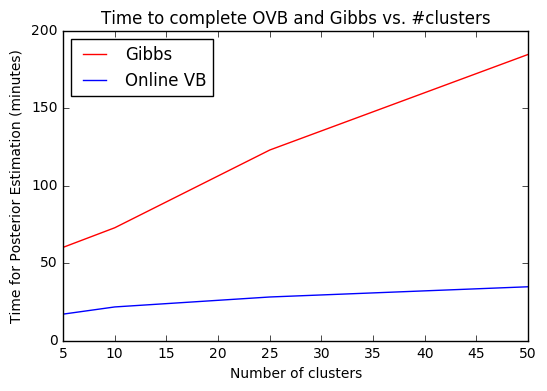
\includegraphics[width=0.5\textwidth]{time}
    \caption{Comparison of the running times of each of the posterior estimation methods across various numbers of topics.}
    \label{fig:time}
\end{figure}

\begin{figure}
    \centering
    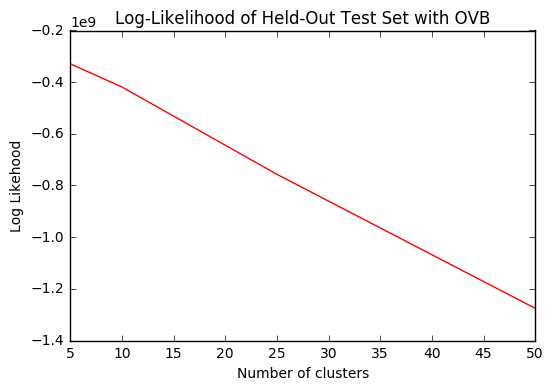
\includegraphics[width=0.5\textwidth]{ll}
    \caption{Log-likelihood of the held-out testing set, across various numbers of topics.}
    \label{fig:ll}
\end{figure}

\begin{figure}
    \centering
    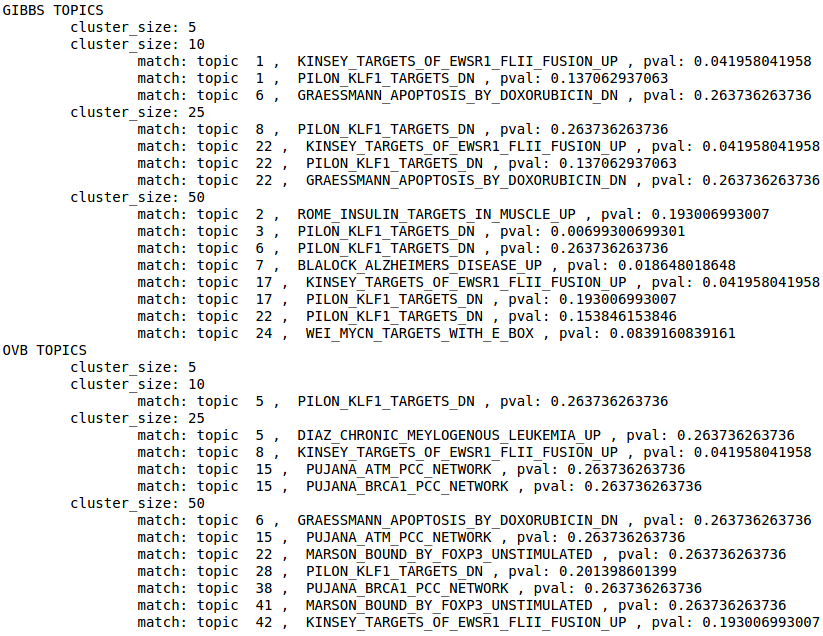
\includegraphics[width=1\textwidth]{pathways}
    \caption{Matches between the gene collections found in LDA topics and published gene sets in \texttt{MSigDB}. Cluster size refers to the number of topics in the model}
    \label{fig:pathways}
\end{figure}

\begin{figure}
    \centering
    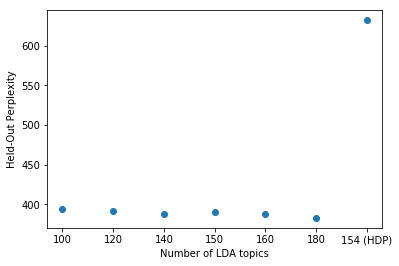
\includegraphics[width=0.5\textwidth]{hdp-perplexity}
    \caption{Comparison of log-likelihood of the held-out testing set, under various LDA models and the HDP model.}
    \label{fig:hdp-perplexity}
\end{figure}

\begin{figure}
    \centering
    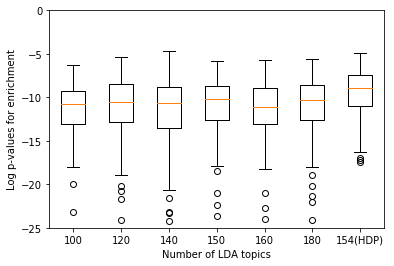
\includegraphics[width=0.5\textwidth]{hdp-enrichment}
    \caption{Comparison of distributions of p-values from gene set enrichment analysis between LDA models and the HDP model.}
    \label{fig:hdp-enrichment}
\end{figure}

\begin{figure}
    \centering
    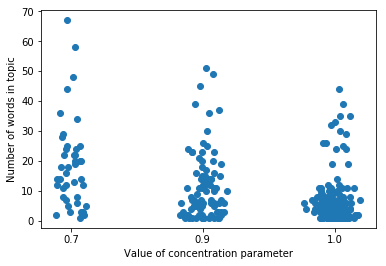
\includegraphics[width=0.5\textwidth]{ibp_words_in_topic}
    \caption{Beeswarm plot of number of words per topic, for 3 different IBP-DP models with different concentration parameters. Each point represents one topic from its model}
    \label{fig:ibp_words_in_topic}
\end{figure}

\begin{figure}
    \centering
    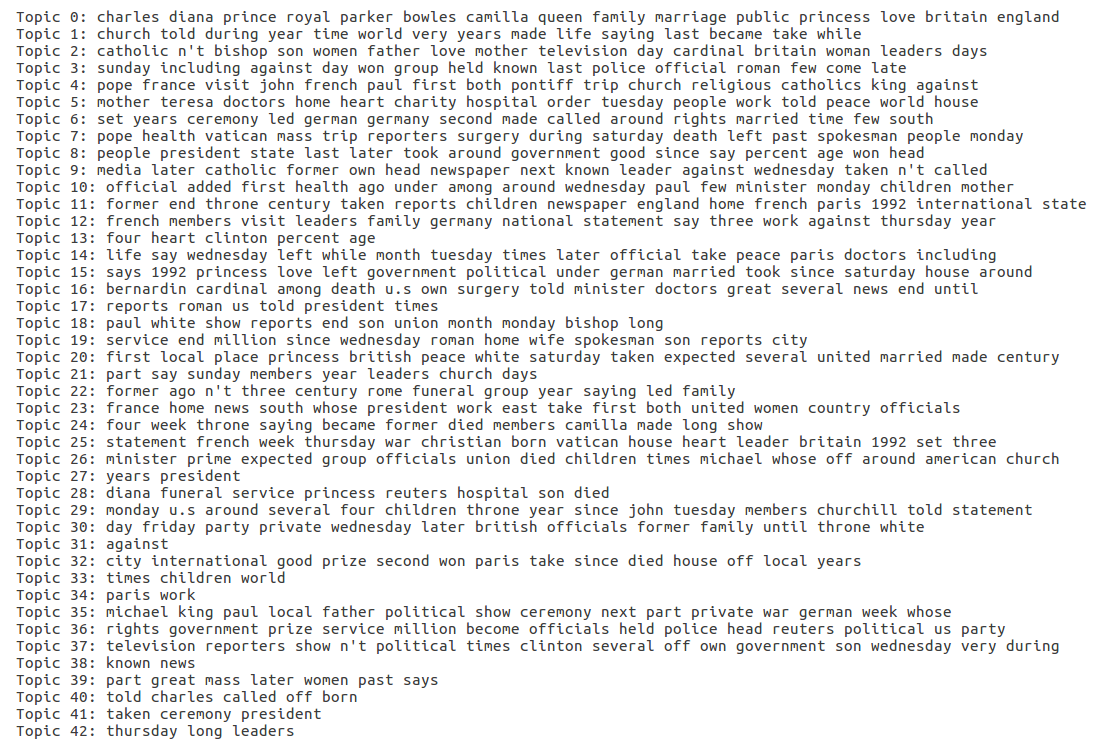
\includegraphics[width=1\textwidth]{ibptopics}
    \caption{Topics from IBP-DP model trained on subset of Reuters dataset.}
    \label{fig:ibptopics}
\end{figure}

\begin{figure}
    \centering
    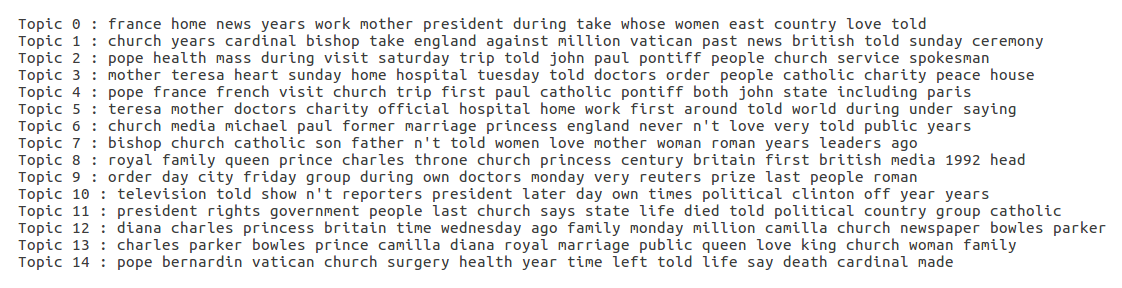
\includegraphics[width=1\textwidth]{ldatopics}
    \caption{Topics from LDA model with 15 topics trained on subset of Reuters dataset.}
    \label{fig:ldatopics}
\end{figure}

\begin{figure}
    \centering
    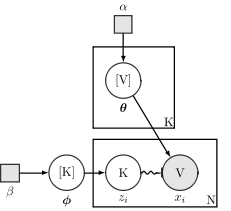
\includegraphics[width=0.3\textwidth]{mixture}
    \caption{Finite \texttt{K}-sized mixture model currently implemented. $\theta$ is the parameter for every cluster component, represented from a categorical draw of over all genes. $z_i$ is the cluster assignment, and $\phi$ is the distribution of clusters. As usual, $\alpha, \beta$ are hyper-parameters.}
    \label{fig:plate}
\end{figure}

\begin{thebibliography}{9}
    \bibitem{hg} 
        The XL-mHG Test For Enrichment: A Technical Report.
        \url{https://arxiv.org/pdf/1507.07905.pdf}
         
    \bibitem{msigdb} 
        Molecular Signatures Database v6.0.
        \url{http://software.broadinstitute.org/gsea/msigdb}
         
    \bibitem{lda} 
        lda: Topic modeling with latent Dirichlet Allocation.
        \url{http://pythonhosted.org/lda/}

    \bibitem{ovb} 
        Online Latent Dirichlet Allocation with variational inference.
        \url{https://github.com/scikit-learn/scikit-learn/blob/master/sklearn/decomposition/online_lda.py}

    \bibitem{plda} 
        C++ implementation of Latent Dirichlet Allocation
        \url{https://github.com/openbigdatagroup/plda/blob/master/lda.cc}

    \bibitem{online}
        Online Learning for Latent Dirichlet Allocation.
        \url{https://pdfs.semanticscholar.org/157a/ef34d39c85d6576028f29df1ea4c6480a979.pdf}

    \bibitem{HDP}
        Hierarchical Dirichlet Processes
        \url{http://people.eecs.berkeley.edu/~jordan/papers/hdp.pdf}

    \bibitem{IBP}
        The IBP Compound Dirichlet Process and its Application to Focused Topic Modeling
        \url{http://www.cs.columbia.edu/~blei/papers/WilliamsonWangHellerBlei2010.pdf}

    \bibitem{TS-DDP}
        A Time-Series DDP for Functional Proteomics Profiles
        \url{https://www.ma.utexas.edu/users/pmueller/pap/NM12.pdf}

    \bibitem{IBP2}
        Stick-breaking Construction for the Indian Buffet Process
        \url{http://mlg.eng.cam.ac.uk/zoubin/papers/TehGorGha07.pdf}

    \bibitem{seurat}
        Spatial reconstruction of single-cell gene expression data
        \url{http://www.nature.com/nbt/journal/v33/n5/full/nbt.3192.html}


\end{thebibliography}


\end{document}
